=\documentclass[14pt,final,oneside]{extarticle}% класс документа, характеристики
%>>>>> Разметка документа
\usepackage[a4paper, mag=1000, left=3cm, right=1.5cm, top=2cm, bottom=2cm, headsep=0.7cm, footskip=1cm]{geometry} % По ГОСТу: left>=3cm, right=1cm, top=2cm, bottom=2cm,
\linespread{1} % межстройчный интервал по ГОСТу := 1.5
%<<<<< Разметка документа
\usepackage[utf8]{inputenc}
\usepackage[T2A]{fontenc}
\usepackage[english, russian]{babel}
\usepackage{amsmath, amsfonts, amssymb, amssymb, amsthm, mathtools}
\usepackage{geometry}
\usepackage{colortbl} % таблички
\usepackage{listings} % листинг
\usepackage{dcolumn} % выравнивание чисел
\usepackage[normalem]{ulem} % для подчёркиваний uline
\ULdepth = 0.16em % расстояние от линии до текста выше/ниже
\lstset{basicstyle=\ttfamily\normalsize}  
\usepackage{graphicx}
\usepackage{longtable}
\usepackage[breaklinks]{hyperref}
\usepackage{xcolor}
\setlength{\parindent}{0pt}
\setlength{\parskip}{6pt}
\usepackage{float}
\makeatletter
\def\cyrrange#1-#2{%
    \begingroup
    \count@=`#1
    \loop
    \lst@literate{\char\count@}{\char\count@}1
    \ifnum\count@<`#2
    \advance\count@\@ne
    \repeat
    \endgroup
}
\makeatother
\lstset{
    inputencoding=utf8,       % Указываем кодировку входного текста
    extendedchars=true,       % Включаем поддержку расширенных символов
    literate=%                % Настройка отображения кириллических символов
        {а}{{\selectfont а}}1
        {б}{{\selectfont б}}1
        {в}{{\selectfont в}}1
        {г}{{\selectfont г}}1
        {д}{{\selectfont д}}1
        {е}{{\selectfont е}}1
        {ё}{{\selectfont ё}}1
        {ж}{{\selectfont ж}}1
        {з}{{\selectfont з}}1
        {и}{{\selectfont и}}1
        {й}{{\selectfont й}}1
        {к}{{\selectfont к}}1
        {л}{{\selectfont л}}1
        {м}{{\selectfont м}}1
        {н}{{\selectfont н}}1
        {о}{{\selectfont о}}1
        {п}{{\selectfont п}}1
        {р}{{\selectfont р}}1
        {с}{{\selectfont с}}1
        {т}{{\selectfont т}}1
        {у}{{\selectfont у}}1
        {ф}{{\selectfont ф}}1
        {х}{{\selectfont х}}1
        {ц}{{\selectfont ц}}1
        {ч}{{\selectfont ч}}1
        {ш}{{\selectfont ш}}1
        {щ}{{\selectfont щ}}1
        {ъ}{{\selectfont ъ}}1
        {ы}{{\selectfont ы}}1
        {ь}{{\selectfont ь}}1
        {э}{{\selectfont э}}1
        {ю}{{\selectfont ю}}1
        {я}{{\selectfont я}}1
        {Б}{{\selectfont Б}}1
        {К}{{\selectfont К}}1
        {О}{{\selectfont О}}1,
    language=Python,            % Язык программирования
    numbers=left,             % Нумерация строк слева
    stepnumber=1,             % Каждая строка нумеруется
    numbersep=5pt,            % Отступ от кода до номеров строк
    showspaces=false,         % Не показывать пробелы
    showstringspaces=false,   % Не показывать пробелы в строках
    tabsize=4,                % Размер табуляции
    frame=single,             % Рамка вокруг кода
    breaklines=true,          % Перенос строк
    breakatwhitespace=false,  % Переносить строки по пробелам
    basicstyle=\ttfamily,     % Шрифт текста
    keywordstyle=\color{blue},% Цвет ключевых слов
    commentstyle=\color{green},% Цвет комментариев
    stringstyle=\color{red},  % Цвет строковых литералов
}
\usepackage{minted} 

\usepackage{titlesec}
\titleformat{\section}
{\LARGE\bfseries}
{\thesection}{15pt}{} 
\usepackage{fancyhdr}
\renewcommand{\thesection}{\arabic{section}.}
\renewcommand{\thesubsection}{\arabic{section}.\arabic{subsection}.}
\usepackage{tocloft}
\renewcommand{\cftsecleader}{\cftdotfill{\cftdotsep}}
\renewcommand{\cftsecfont}{\Large\bfseries} 
\renewcommand{\cfttoctitlefont}{\LARGE\bfseries}
\newcommand{\lr}[1]{\left( {#1} \right)}
\usepackage{hyperref} % гиперссылки
\hypersetup{
    colorlinks=true,        % Включаем цветные ссылки
    linkcolor=blue!50!black, % Цвет внутренних ссылок (например, на разделы)
    urlcolor=blue!50!black,  % Цвет URL-ссылок
    citecolor=blue!50!black, % Цвет ссылок на библиографию
}
\usepackage{tikz}

% Команда для обведенного знака равенства
\newcommand{\circledequal}{%
    \mathbin{%
        \tikz[baseline=(X.base)] 
            \node[draw, circle, inner sep=0pt] (X) {$=$};%
    }%
}

\graphicspath{{analysis/figures/}}
\setlength{\emergencystretch}{2em}
\renewcommand{\arraystretch}{1.2}
\newcommand{\studentgroup}{P3309}
\newcommand{\examiner}{Смирнов Виктор Игоревич}

\newcommand{\ratioRW}{67.65}
\newcommand{\ratioMmap}{1.73}
\newcommand{\ratioCacheMethods}{41.71}

\begin{document}
\hypersetup{pageanchor=false}
\begin{titlepage}
\thispagestyle{empty}
\begin{center}
\LARGE Университет ИТМО
\vspace{20pt}

\Large Факультет программной инженерии и компьютерной техники\\
Образовательная программа\linebreak
«Системное и прикладное программное обеспечение»
\vfill

\LARGE Лабораторная работа\\
\Large по дисциплине «Операционные системы»\\[12pt]
Экспериментальное введение в курс\\[12pt]
\normalsize Вариант: Write, Cache/NoCache, 10M, Rand
\vfill
\end{center}
\begin{flushright}
\large Выполнил студент группы \studentgroup\\
Евграфов Артём Андреевич\\[12pt]
Проверил: \examiner
\end{flushright}
\vfill
\begin{center}
\large Санкт-Петербург 2026
\end{center}
\end{titlepage}

\setcounter{page}{1}
\hypersetup{pageanchor=true}
\tableofcontents
\newpage

\section{Цель и задание}
Цель работы - экспериментально сравнить время обхода и обновления
записей бинарного файла при разных способах доступа к файлу и режимах
работы с системным файловым кэшем, освоить
воспроизводимую постановку эксперимента и статистическую обработку
измерений.

Вариант \textbf{Write, Cache/NoCache, 10M, Rand} фиксирует режим
обновления данных, целевой размер файла 10~МиБ и случайный физический
порядок обхода. Сравниваемый фактор - наличие флага
\texttt{--no-cache} при запуске каждой из двух программ.

\begin{itemize}
\item \texttt{graph\_traverse}: доступ через \texttt{lseek()},
\texttt{read()} и \texttt{write()}.
\item \texttt{graph\_traverse\_mmap}: отображение файла в память
через \texttt{mmap()} и работа с записями по адресам памяти.
\end{itemize}

Обе программы обходят цепочку вершин. Каждая вершина содержит значение
и индекс следующей вершины. В режиме \texttt{--write} программа сначала
читает запись, затем увеличивает её значение на единицу. Таким образом,
исследуется нагрузка чтения с обновлением, а не изолированная запись.

\begin{center}
\small
\begin{tabular}{|l|l|l|}
\hline
Серия & Программа & Флаги\\ \hline
A & \texttt{graph\_traverse} & \texttt{--write}\\ \hline
B & \texttt{graph\_traverse} & \texttt{--write --no-cache}\\ \hline
C & \texttt{graph\_traverse\_mmap} & \texttt{--write}\\ \hline
D & \texttt{graph\_traverse\_mmap} & \texttt{--write --no-cache}\\ \hline
\end{tabular}
\end{center}

Во всех четырёх сериях используется случайный граф одинакового размера.
Порядок обхода не является изменяемым фактором данного варианта.

\subsection{Особенности реализации Cache/NoCache}
В режиме \texttt{--no-cache} программа \texttt{graph\_traverse}
использует на Linux флаг \texttt{O\_DIRECT} при открытии файла.
Обход файлового кэша требует выравнивания адресов, смещений и размеров
операций. Реализация читает охватывающий блок, а для обновления значения
выполняет чтение, изменение и запись блока. Поэтому меняются не только
правила кэширования, но и объём передаваемых данных.

Для \texttt{mmap} флаг \texttt{--no-cache} имеет иной смысл:
файловый кэш сохраняется, а \texttt{madvise(MADV\_RANDOM)} задаёт
рекомендацию по упреждающему чтению. После обновления выполняются
\texttt{msync(MS\_SYNC)} и
\texttt{madvise(}\allowbreak\texttt{MADV\_DONTNEED)}.
Последняя рекомендация не гарантирует удаления страниц из файлового
кэша. При этом время синхронной обратной записи входит во время
запуска серии~D. В серии~C явного \texttt{msync(MS\_SYNC)} нет.
Данные различия необходимо учитывать при интерпретации результатов.

\section{Подготовка программ и данных}
Обе программы собраны GCC 13.3.0 без дополнительных флагов оптимизации:
{\small
\begin{verbatim}
mkdir -p out
gcc -o out/graph_traverse src/graph_traverse.c
gcc -o out/graph_traverse_mmap \
  src/graph_traverse_mmap.c
\end{verbatim}
}
Параметры генерации случайного графа:
{\small
\begin{verbatim}
python3 graphgen.py -s 10M --seed 427 \
  --topology chain -b 0.5 --min-step-pages 2 \
  --verify -o graph-rand.bin
\end{verbatim}
}
Зерно 427 фиксирует исходную генерацию. Топология \texttt{chain}
задаёт цепочку со случайным физическим порядком вершин. В основных
сериях данного варианта сравнивается режим Cache/NoCache на одном
случайном графе. Последовательный граф не является вторым сравниваемым
фактором; скрипт \path{generate.sh} также позволяет создать его для
ознакомления и воспроизведения общей методички.

\begin{center}
\small
\begin{tabular}{|l|r|}
\hline
Параметр & Значение\\ \hline
Размер файла, байт & 10\,485\,760\\ \hline
Число записей & 436\,905\\ \hline
Размер записи / заголовка, байт & 24 / 40\\ \hline
Индекс начальной вершины & 252\,929\\ \hline
Исходящих рёбер на вершину, не более & 1\\ \hline
\end{tabular}
\end{center}
При обработке отдельно проверены структура и достижимость всех
436\,905 вершин, отсутствие повторных посещений и корректное завершение
цепочки. Получены 218\,081 переход вперёд и 218\,823 назад.
Доля переходов короче 342 записей составляет 0.436\%.
Это согласуется с преимущественно удалёнными переходами.
Пересечение границ страниц само по себе не гарантирует промах
файлового кэша.

Скрипт сбора повторно использует файл: каждый полный запуск увеличивает
значения, сохраняя ссылки, размер и порядок обхода. Граф перед каждым
измерением заново не генерируется. Проверка структуры при обработке
не изменяет исходный файл. Её результат и хеш структуры без изменяемых
полей сохранены в \path{analysis/summary.json}.

\section{Стенд и настройка окружения}
Сведения перед основной серией сохранены в журнале
\path{results/environment-before-main.txt};
снимок после серии - в \path{results/environment-after-main.txt}.
Каталог результатов далее указывается относительно папки лабораторной.

\begin{center}
\small
\begin{tabular}{|p{4.2cm}|p{10.3cm}|}
\hline
Параметр & Наблюдаемое значение\\ \hline
Система & Ubuntu 24.04.4 LTS, x86\_64; дистрибутив уточнён
по \path{/etc/os-release} при обработке\\ \hline
Ядро основных серий & 7.0.0-38-generic\\ \hline
CPU & Intel Core i7-11370H; 4 ядра, 8 логических CPU\\ \hline
Кэши CPU & L1d 192~КиБ, L1i 128~КиБ, L2 5~МиБ суммарно;
L3 12~МиБ общий\\ \hline
RAM до серии & 15\,771.1~МиБ; доступно около 12~ГиБ\\ \hline
Подкачка & 4~ГиБ; занято до серии около 2.6~ГиБ,
после - около 2.9~ГиБ\\ \hline
Накопитель & \texttt{nvme0n1}, «PCIe-8 SSD 1TB» по
\texttt{lsblk}, 953.9~ГиБ, \texttt{ROTA=0}\\ \hline
Файловая система графа & ext4, \texttt{/dev/nvme0n1p8},
основной раздел \texttt{/}; подтверждено \texttt{findmnt}\\ \hline
Инструменты & GCC 13.3.0, Python 3.12.3, perf 7.0.14\\ \hline
Виртуализация & \texttt{systemd-detect-virt}: \texttt{none}\\ \hline
\end{tabular}
\end{center}

Перед пилотом установлен governor \texttt{performance}.
На снимке перед основной серией частота логических CPU составляла
около 4.3~ГГц; это наблюдение, а не гарантия постоянной частоты.
Режим не отменяет динамическое управление и температурные ограничения.
Turbo Boost не отключался: при дополнительной проверке
\path{intel_pstate/no_turbo} имел значение 0.

Каждая исследуемая программа закреплялась на логическом CPU~2.
Пары потоков одного физического ядра: (0,4), (1,5), (2,6), (3,7).
Поток~6 и фоновые задачи не изолировались. Загрузка системы была
ненулевой: load average за минуту до серии 1.74, после - 2.09;
доля простоя CPU на снимках около 79\% и 77\%. Системные параметры
не менялись внутри основных серий, но полностью устранить помехи
на рабочем компьютере не удалось.

Файл 10~МиБ существенно меньше доступной RAM и помещается в файловый
кэш. Поэтому выбран контролируемый прогрев, а не увеличение данных
до размера больше RAM. Кэши L1/L2/L3 и файловый кэш различаются.
Температура и троттлинг непрерывно не регистрировались.

\section{Гипотезы и методика}
До основной серии сформулированы гипотезы:
обычный обход с файловым кэшем быстрее прямого ввода-вывода;
для \texttt{mmap} флаг \texttt{--no-cache} увеличивает время,
в частности из-за синхронной обратной записи. 

\subsection{План и границы измерения}
Основная метрика - полное время отдельного запуска, включая создание
процесса, \texttt{taskset}, открытие файла, один обход с обновлением
и завершение. Использован \texttt{collect.py} и монотонный
\texttt{perf\_counter\_ns}; наносекундные единицы не означают такую же
экспериментальную точность.

Перед каждым запуском родительский процесс выполняет
\texttt{fsync} файла и полное обычное чтение кусочками по 1~МиБ.
Это подготовка вне таймера: предыдущее изменение синхронизируется,
а данные прогреваются по одному правилу. У \texttt{O\_DIRECT}
предварительное чтение не отменяет прямой путь доступа. Глобальный
сброс кэшей не применяется. Время последующей синхронизации обычной
записи не добавляется к предыдущему запуску; результат не является
сравнением одинаковых гарантий сохранности данных.

Один круг содержит четыре запуска A--D, последовательно.
Начальная конфигурация циклически сдвигается:
ABCD, BCDA, CDAB, DABC. Это уменьшает привязку режима к позиции
в серии. Внутри запуска один обход (\texttt{ITER=1}).
Прогревочные чтения исключены по построению; ни первые наблюдения,
ни большие времена из CSV не удалялись.

Пилот содержит 6 запусков каждого режима, основная серия - 30,
всего 120 наблюдений. Все коды завершения нулевые; журналы подтверждают
обработку 436\,905 записей каждым запуском. Метаданные, команды и
показатели отдельных процессов сохранены. Статистика детей получена
как разность \texttt{getrusage(RUSAGE\_CHILDREN)} до и после одного
дочернего запуска; подготовка родительского Python в неё не входит.

\subsection{Обоснование числа повторов}
После пилота выбран ориентир: полуширина 95\%-го интервала не более
10\% среднего. Для обычного режима с кэшем пилот дал
$\bar t=1.0423$~с, $s=0.2544$~с. Первое приближение:
\[
N\approx\left(\frac{1.96s}{0.1\bar t}\right)^2\approx23.
\]
Выбрано $N=30$ с запасом, общее для четырёх конфигураций.

\subsection{Статистическая обработка}
Для каждой серии вычислены выборочное среднее, стандартное отклонение
со знаменателем $N-1$ и приближённый t-интервал среднего:
\[
\bar t=\frac1N\sum t_i,\qquad
s=\sqrt{\frac1{N-1}\sum(t_i-\bar t)^2},\qquad
\bar t\pm t_{0.975,N-1}\frac{s}{\sqrt N}.
\]

Гистограмма группирует наблюдения по интервалам; KDE даёт сглаженную
оценку плотности, зависящую от ширины сглаживания (правило Scott).
Для далеко разнесённых времён обычного обхода показана плотность
$\log_{10}(t/\text{с})$, для \texttt{mmap} - плотность времени
в миллисекундах. Все исходные точки сохранены.

\section{Результаты основных серий}
Обработаны 120 успешных запусков: по 30 в каждой серии A--D.
Сырые измерения сохранены в \path{results/main/measurements.csv};
пилотные и диагностические результаты к этой таблице не добавлялись.
Ни одно наблюдение основной серии не исключено.

\begin{center}\small
\begin{tabular}{|c|r|r|r|c|r|}\hline
Серия & $N$ & Среднее, с & $s$, с & 95\% ДИ, с & $E/\bar t$, \%\\ \hline
A & 30 & 0.874828 & 0.104919 & [0.835650; 0.914005] & 4.48 \\ \hline
B & 30 & 59.182591 & 4.187805 & [57.618839; 60.746343] & 2.64 \\ \hline
C & 30 & 0.020972 & 0.003712 & [0.019586; 0.022358] & 6.61 \\ \hline
D & 30 & 0.036247 & 0.023247 & [0.027566; 0.044927] & 23.95 \\ \hline
\end{tabular}\end{center}

Здесь $s$ - выборочное стандартное отклонение, $E$ - полуширина
t-интервала. По средним обычный обход с флагом
\texttt{--no-cache} медленнее в \ratioRW{} раза,
а \texttt{mmap} - в \ratioMmap{} раза.
Среднее время обычного обхода с кэшем больше времени \texttt{mmap}
с кэшем в \ratioCacheMethods{} раза.

\begin{figure}[htbp]
\centering
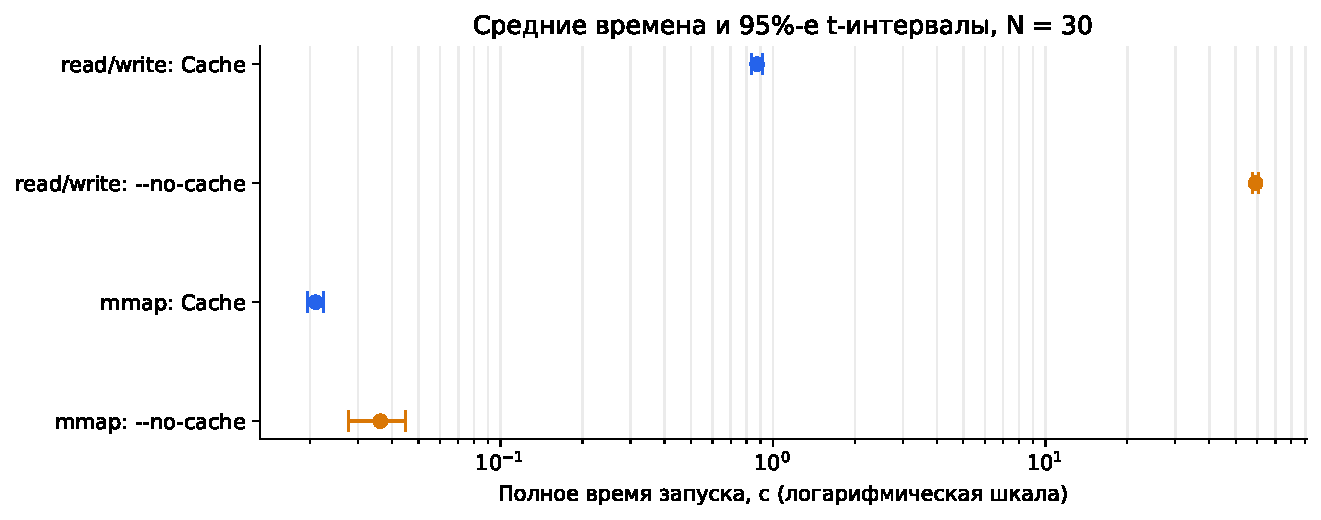
\includegraphics[width=\linewidth]{means.pdf}
\caption{Четыре средних времени с 95\%-ми t-интервалами.
Логарифмическая шкала позволяет показать все серии на одном графике.}
\end{figure}

У обычного обхода без кэша среднее CPU-время составляет около 5.00~с
при wall time 59.18~с. Около 54.18~с процесс не исполнялся на CPU.
Это согласуется с длительными ожиданиями ввода-вывода, но по разности
времён нельзя отделить все причины ожидания.
У обычного обхода с кэшем CPU-время почти равно полному времени,
причём около 86\% CPU-времени приходится на ядро ОС.

\begin{center}\small
\begin{tabular}{|c|r|r|r|r|r|r|}\hline
Серия & User, с & Sys, с & Vol. ctx & Invol. ctx & Minor & Major\\ \hline
A & 0.1253 & 0.7481 & 1.23 & 39.93 & 135.70 & 0.10 \\ \hline
B & 0.4605 & 4.5394 & 1\,324\,375.40 & 49.83 & 136.37 & 0.00 \\ \hline
C & 0.0166 & 0.0041 & 1.10 & 3.20 & 2779.77 & 0.07 \\ \hline
D & 0.0165 & 0.0041 & 5.03 & 2.80 & 2779.50 & 0.00 \\ \hline
\end{tabular}\end{center}

В таблице приведены средние показатели отдельных запусков.
Обычное чтение использует небольшой повторно используемый буфер;
\texttt{mmap} отображает страницы файла и имеет существенно больше
minor faults.

\subsection{Распределения и устойчивость}
В основной серии диапазоны времён составили:
A - 0.819--1.379~с, B - 57.026--70.179~с,
C - 17.762--30.507~мс, D - 21.830--98.032~мс.
У серии D медиана 27.10~мс ниже среднего 36.25~мс;
редкие задержки образуют правый хвост. Видны и отдельные повышенные
значения в остальных сериях. Плотности не дают основания автоматически
считать исходные распределения нормальными.

\begin{figure}[htbp]
\centering
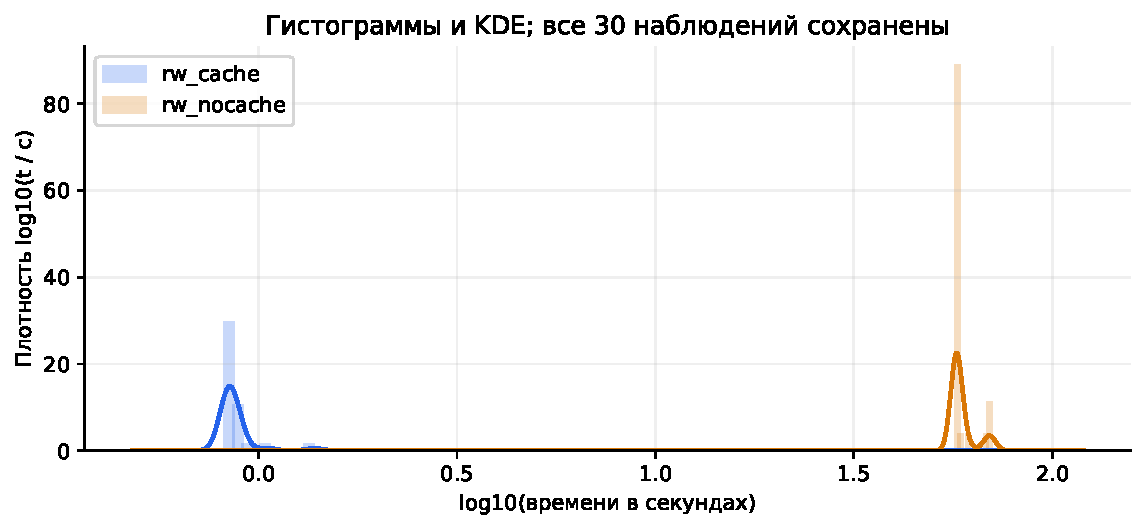
\includegraphics[width=.97\linewidth]{distribution_rw.pdf}
\par\medskip
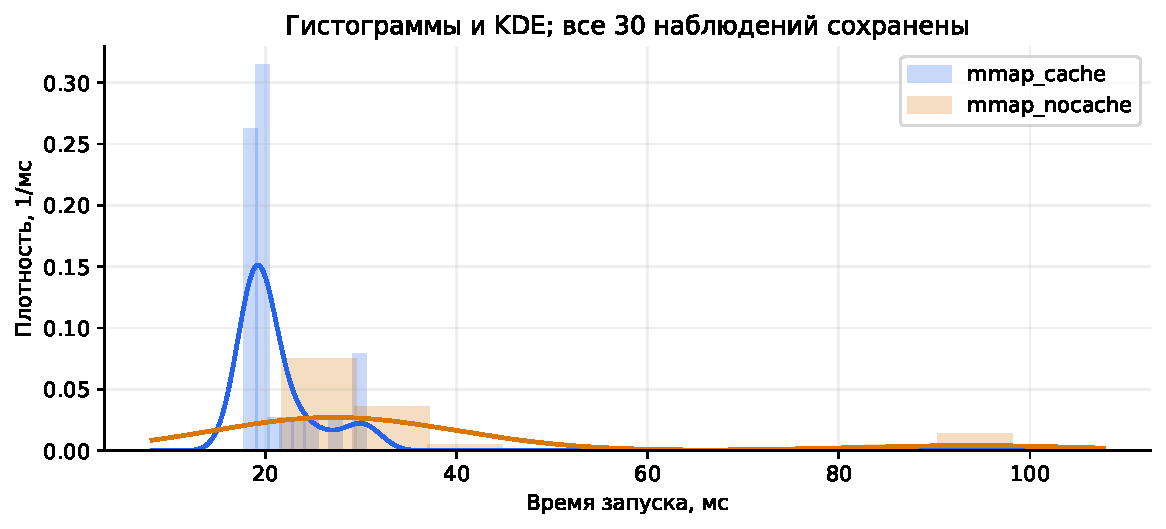
\includegraphics[width=.97\linewidth]{distribution_mmap.pdf}
\caption{Совмещённые гистограммы и KDE для сравниваемых режимов.
Верхний график показывает плотность логарифма времени обычного обхода;
нижний - плотность времени \texttt{mmap} в миллисекундах.}
\end{figure}

\begin{figure}[htbp]
\centering
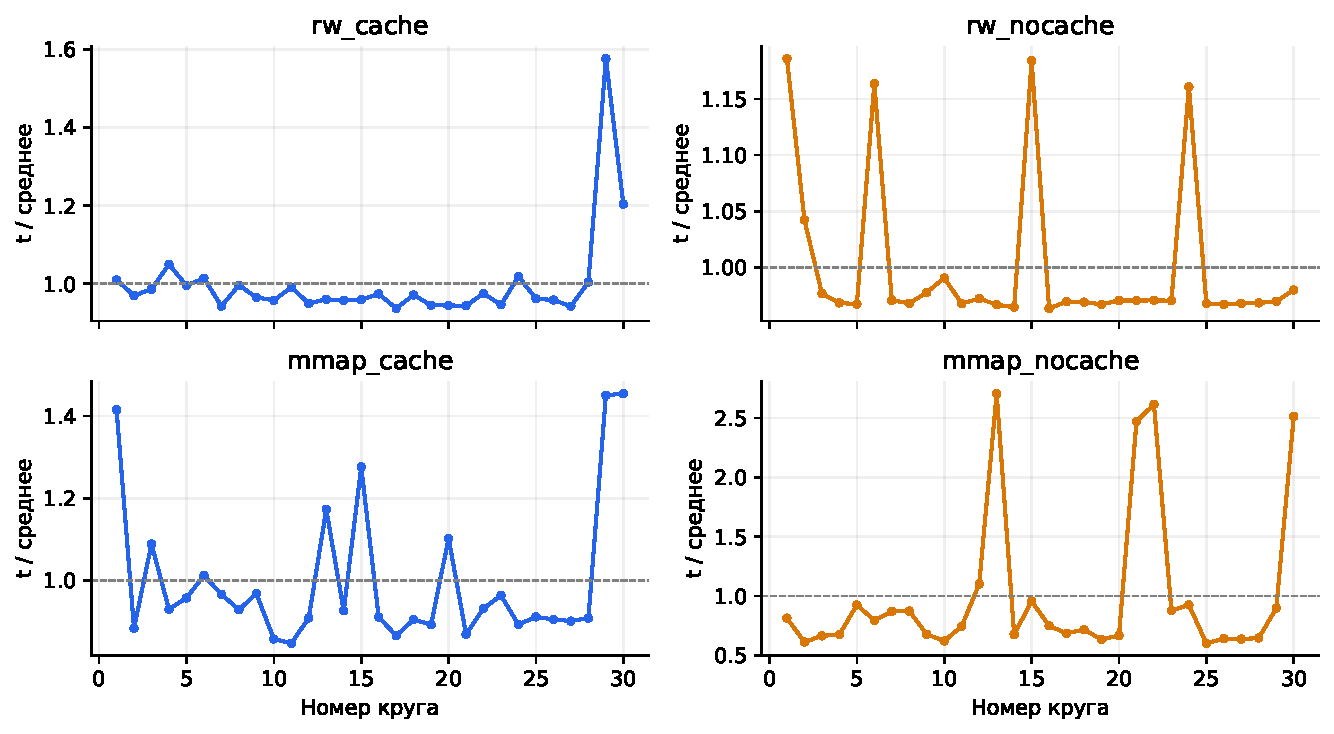
\includegraphics[width=\linewidth]{runs.pdf}
\caption{Время каждого запуска относительно среднего своей серии.
Все наблюдения, включая повышенные значения, сохранены.}
\end{figure}

\subsection{Достаточность измерений}
Относительные полуширины интервалов составили 4.48\%, 2.64\%,
6.61\% и 23.95\%. Ориентир 10\% достигнут в A--C.
В D точность ниже целевой. При сохранении текущего разброса формула даёт
около 159 наблюдений для D; уточнение t-квантили - около 161,
то есть примерно на 131 больше текущего числа.

Дополнительные измерения именно быстрых режимов \texttt{mmap}
эффективнее повторения всех дорогих кругов.
Оценка требуемого N приблизительна: при изменении разброса
она изменится. В общем случае для уменьшения полуширины вдвое
при неизменных условиях потребуется примерно вчетверо больше наблюдений.

\section{Диагностика и влияние инструментов}
Перед диагностическими запусками выполнялись синхронизация файла и
прогрев по тому же принципу. Эти результаты не включены в основные
серии. На каждом инструментированном запуске обработаны все вершины.

\subsection{Системные вызовы и strace}
\begin{center}
\small
\begin{tabular}{|c|r|r|r|r|r|}
\hline
Серия & read & write & lseek & Всего & Wall, с\\ \hline
A & 436\,908 & 436\,907 & 873\,811 & 1\,747\,694 & 21.66\\ \hline
B & 887\,466 & 436\,907 & 1\,324\,369 & 2\,648\,814 & 86.75\\ \hline
C & 2 & 2 & 0 & 74 & 0.03\\ \hline
D & 2 & 2 & 0 & 77 & 0.03\\ \hline
\end{tabular}
\end{center}
Трассировка включает запуск \texttt{taskset} и последующее приложение.
В A число вызовов соответствует чтению, двум позиционированиям
и обновлению на каждую запись. В B дополнительные чтения связаны
с выровненной схемой чтения--изменения--записи и границами блоков.
Для \texttt{mmap} нет системных вызовов на каждую вершину;
единичные read/write относятся к запуску и сообщениям.
В D дополнительно наблюдаются один \texttt{msync} и два
\texttt{madvise}, что подтверждает особенности режима.

С \texttt{strace} обычный кэшированный обход занял 21.66~с
против среднего 0.875~с основной серии - примерно в 24.8 раза
больше. Для B отношение около 1.47.

\subsection{Счётчики perf}
Из-за \texttt{perf\_event\_paranoid=4} команды выполнялись с
\texttt{sudo}; \texttt{taskset} закреплял \texttt{perf} и приложение
на CPU~2 до начала счёта. Исследованы режимы A и C.
\begin{center}
\small
\begin{tabular}{|l|r|r|}
\hline
Показатель & A & C\\ \hline
Context switches & 302 & 24\\ \hline
CPU migrations & 0 & 0\\ \hline
Page faults & 61 & 2\,782\\ \hline
Cache misses & 2\,355\,053 & 733\,292\\ \hline
Полное время, с & 1.0431 & 0.0371\\ \hline
\end{tabular}
\end{center}
Отсутствие миграций согласуется с закреплением CPU.
Больше page faults у \texttt{mmap} соответствует доступу к
страницам отображения. \texttt{Cache-misses} - аппаратный
счётчик промахов кэша CPU, а не число промахов файлового кэша.
Границы счёта отличаются от родительского таймера Python.
Времена с perf выше средних основной серии, но единичный запуск,
изменение привилегий и остаточная нагрузка не позволяют выделить
точные накладные расходы только perf.

\subsection{Фоновая нагрузка}
Контрольная демонстрация выполнялась с тем же обычным кэшированным
обходом. Дополнительный Python-процесс 15 секунд занимал CPU~2.
После прогрева выполнены один запуск без специального конкурента
и один с ним:
\begin{center}
\small
\begin{tabular}{|l|r|r|}
\hline
Показатель & Контроль & С нагрузкой\\ \hline
Wall time, с & 0.96 & 1.98\\ \hline
User + system, с & 0.96 & 0.98\\ \hline
CPU процесса, \% & 99 & 49\\ \hline
Вынужденные переключения & 327 & 533\\ \hline
\end{tabular}
\end{center}
Полное время выросло примерно в 2.06 раза при близком CPU-времени.
Это согласуется с разделением CPU с конкурентом.
Демонстрация имеет N=1 на условие и не является отдельным
статистическим доказательством коэффициента замедления.

\section{Вывод}
На данном Linux-стенде обычное обновление случайных записей без
файлового кэша оказалось в \ratioRW{} раза медленнее кэшированного.
Результат согласуется с гипотезой: схема прямого ввода-вывода
выполняет множество отдельных передач и дополнительные чтения
блоков. Небольшой размер файла не устраняет стоимость количества
операций.

При \texttt{mmap} флаг \texttt{--no-cache} увеличил среднее время
в \ratioMmap{} раза. Направление эффекта согласуется с гипотезой
и наличием синхронной обратной записи. Однако это не полное
отключение файлового кэша, и приписать всю разность одному механизму
по собранным данным нельзя. Сравнение обычного обхода и \texttt{mmap}
относится к готовым реализациям с разными правилами ввода-вывода
и завершения записи, а не к равным гарантиям сохранности.

Критичны были управляемое состояние кэша, фоновая конкуренция
и отделение диагностики от основной серии.
Рабочий набор помещается в RAM; основной эксперимент характеризует
прогретый файловый кэш и прямой путь доступа к SSD.
Модель CPU и диска зафиксирована для воспроизведения, но их
индивидуальное влияние не выделялось отдельным экспериментом.
Поэтому нельзя переносить численные коэффициенты на другие
накопители или объявлять конкретные параметры аппаратуры неважными.

Гипотезы получили поддержку в основных сериях.
Точность оценки достаточна для ориентира 10\% в трёх сериях;
для \texttt{mmap --no-cache} остаётся ограничение около 24\%.
Для уточнения полезны дополнительные короткие измерения и более
строгая изоляция стенда, а не удаление наблюдаемых задержек.
\end{document}
